\problem

\begin{figure}
	\centering
	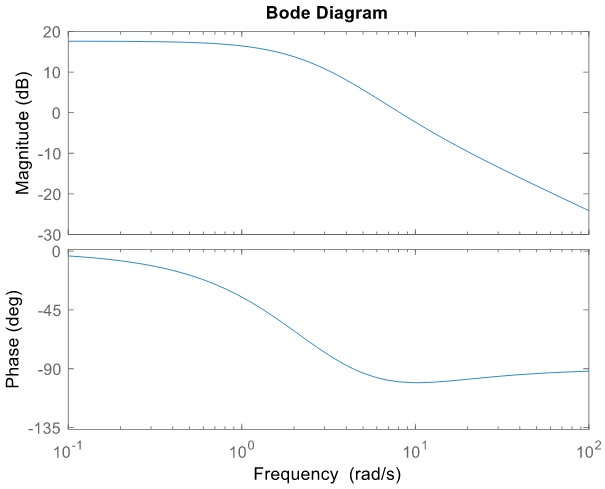
\includegraphics[width=\linewidth]{bode.png}
	\caption{Bode plot of plant.}
	\label{fig:p1:bode}
\end{figure}


From \cref{fig:p1:bode}, the DC gain of the plant appears to be about \SI{17}{\decibel}. This results in the following approximate steady state error:
\begin{align*}
	e &\simeq \frac{1}{1+G_p(0)}\\
	&\simeq \frac{1}{1+10^\frac{17}{20}}\\
	&\simeq 12.4\%
\end{align*}

\subproblem{Margins}

The gain margin is infinite as the phase is never less than $180^\circ$.

The phase at $\omega_gc\simeq\SI{8}{\radian\per\second}$ is $\sim -95^\circ$, therefore the phase margin is $\sim -180^\circ +95^\circ=85^\circ$.\\

\subproblem{Specifications}

\subsubsection*{Closed loop system must be stable}

For the closed loop system to be stable, both gain and phase margins must be positive. As the gain margin is infinite, any increase in gain will not destabilise this system. The phase margin is positive by $85^\circ$, this is a good margin to use during controller design.

\subsubsection*{Steady state error $<5\%$}
The steady state error of the closed loop system to a step input must be less than 5\%. The minimum DC gain of the open loop system to accomplish this is calculated as follows:
\begin{align*}
	G_o(0) &> \frac{1}{e} -1 \\
	&= 19 \simeq \SI{25.6}{\decibel}
\end{align*}
The required controller gain is calculated from the following expression for the open loop gain:
\begin{align*}
	G_o(s) &= G_c(s) + G_p(s)\\
	\iff G_c(0) &= G_o(0) - G_p(0)\\
	&=\SI{25.6}{\decibel} - \SI{17}{\decibel}\\
	&= \SI{8.6}{\decibel}
\end{align*}
I took \SI{10}{\decibel} as the gain to give a margin.

With this controller gain, the open loop dc gain becomes \SI{27}{\decibel}, shifting the gain plot in \cref{fig:p1:bode} up \SI{10}{\decibel}. The gain crossover frequency of the open loop system is about \SI{20}{\radian\per\second} (rising from about \SI{8}{\radian\per\second} in the closed loop system).

\subsubsection*{Percentage overshoot less than 5\%}
Approximating the system as a second order system, the relationship between the percentage overshoot and the damping ratio is given below:
\begin{align*}
	PO & 100\exp{\frac{-\pi \zeta}{\sqrt{1-\zeta^2}}}
\end{align*}
Solving this in \matlab gives a minimum damping ratio of 0.69 for a percentage overshoot of 5\%. To satisfy the specification with a decent margin I chose $\zeta=0.72$.

\subsubsection*{Settling time $t_{s,2\%}\leq \SI{1}{\second}$}
The settling time in relation to the natural frequency and the damping ratio is given by (expression for a second order system):
\begin{align*}
	t_{s,2\%} &\simeq \frac{4}{\zeta \omega_n}\\
	\iff \omega_n &\geq \frac{4}{\zeta t_{s,2\%}}
\end{align*}
Which translates to the following minimum gain crossover frequency:
\begin{align*}
	\omega_gc &\geq \omega_n \sqrt{\sqrt{1 + 4\zeta^4}-2\zeta^2}\\
	&\geq \SI{3.53}{\radian\per\second} 
\end{align*}

\subproblem{Controller}
The controller that satisfies all of these conditions is a lead-lag controller with $\alpha=0$, $\tau=0$ and $k=\SI{10}{\decibel}=3.16$. The gain crossover frequency introduced by the gain satisfies the settling time and percentage overshoot specifications on its own..
$$
G_c(s) = k\text{,}\qquad k=3.16
$$